Удобным для интерпретации является построение трехкристальных карт в обратном пространстве.
Переход в обратное пространство позволяет исключить из рассмотрения особенности
конструкции дифрактометра и типов сканирований, проводимых в эксперименте.
 Угловые положения падающего и дифрагированного пучков
определяют вектор рассеяния $\vec{q}$. Такой вектор можно разложить на составляющие:
$q_z$ - вертикальную составляющую,
направленную перпендикулярно к отражающей атомной плоскости и $q_x$ - горизонтальную составляющую,
лежащую в отражающей плоскости (рис. \ref{ris:q_vector_reciprocal_space}).

\begin{figure}[H]
  \centering
  \subfloat[]{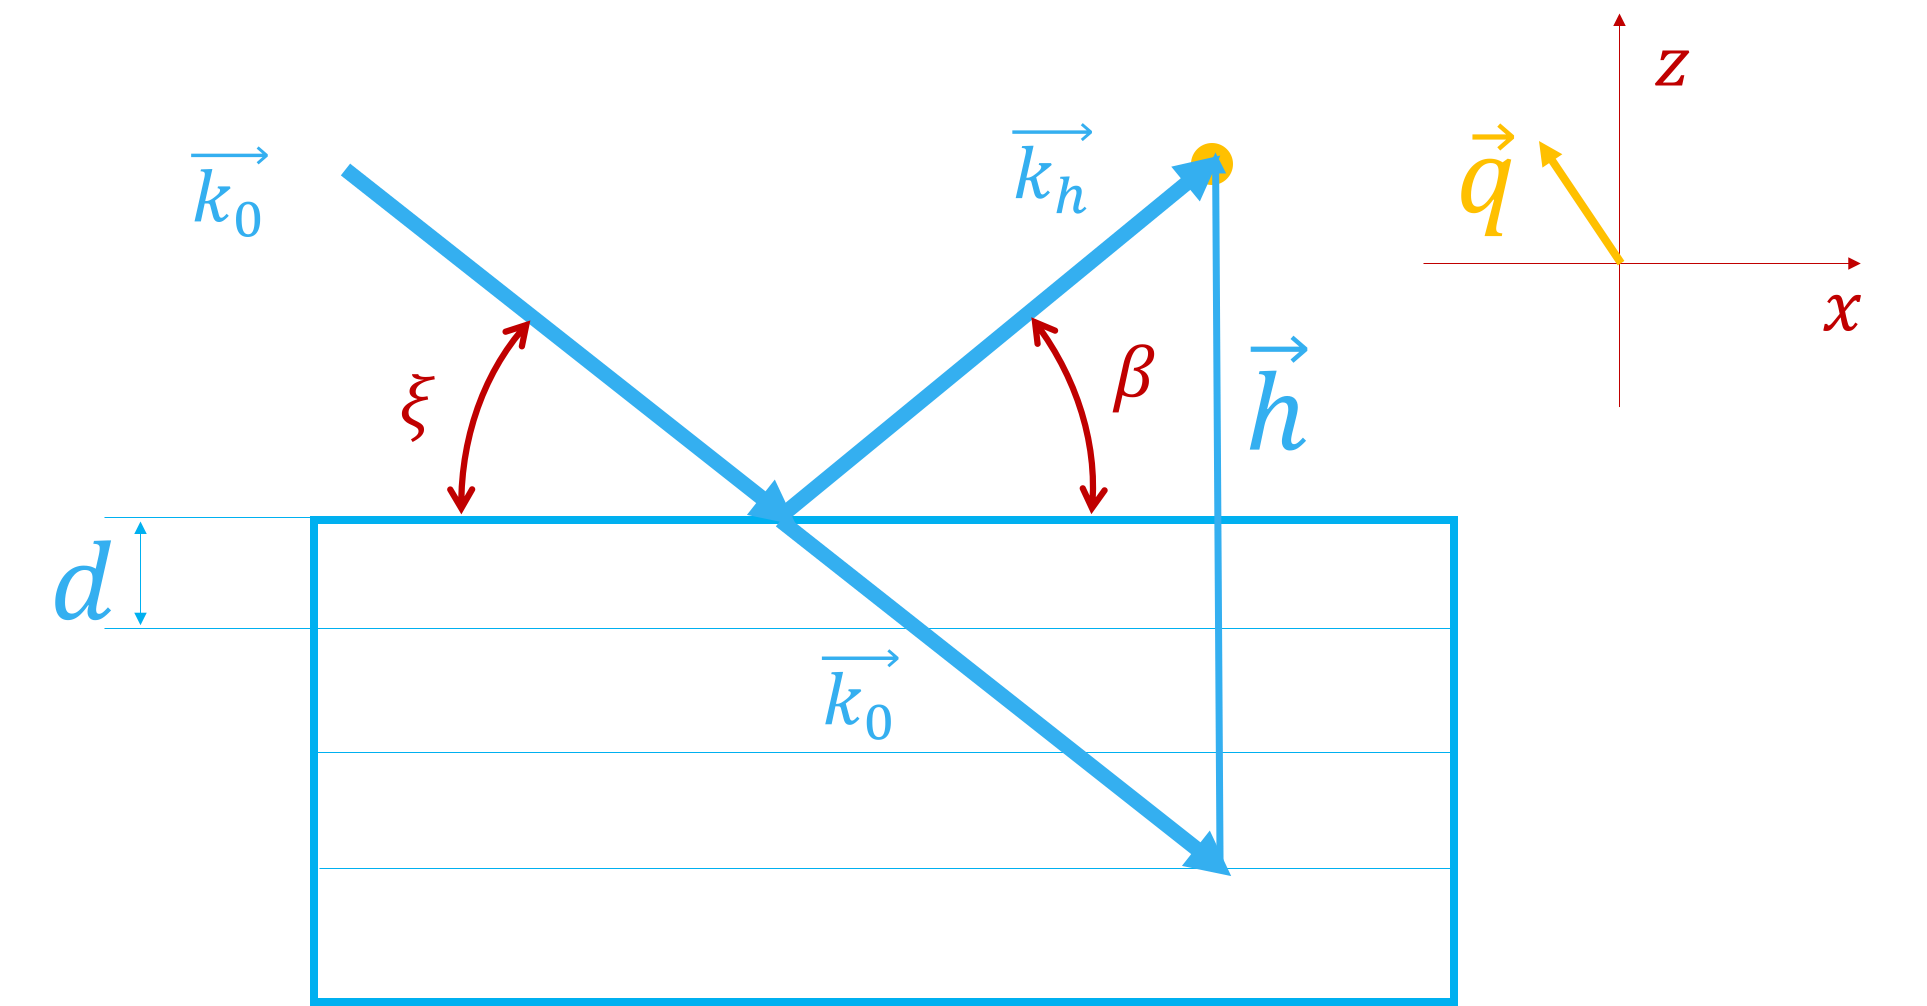
\includegraphics[width=0.3\textwidth]{images/q_vector/0.png}}
  \hfill
  \subfloat[]{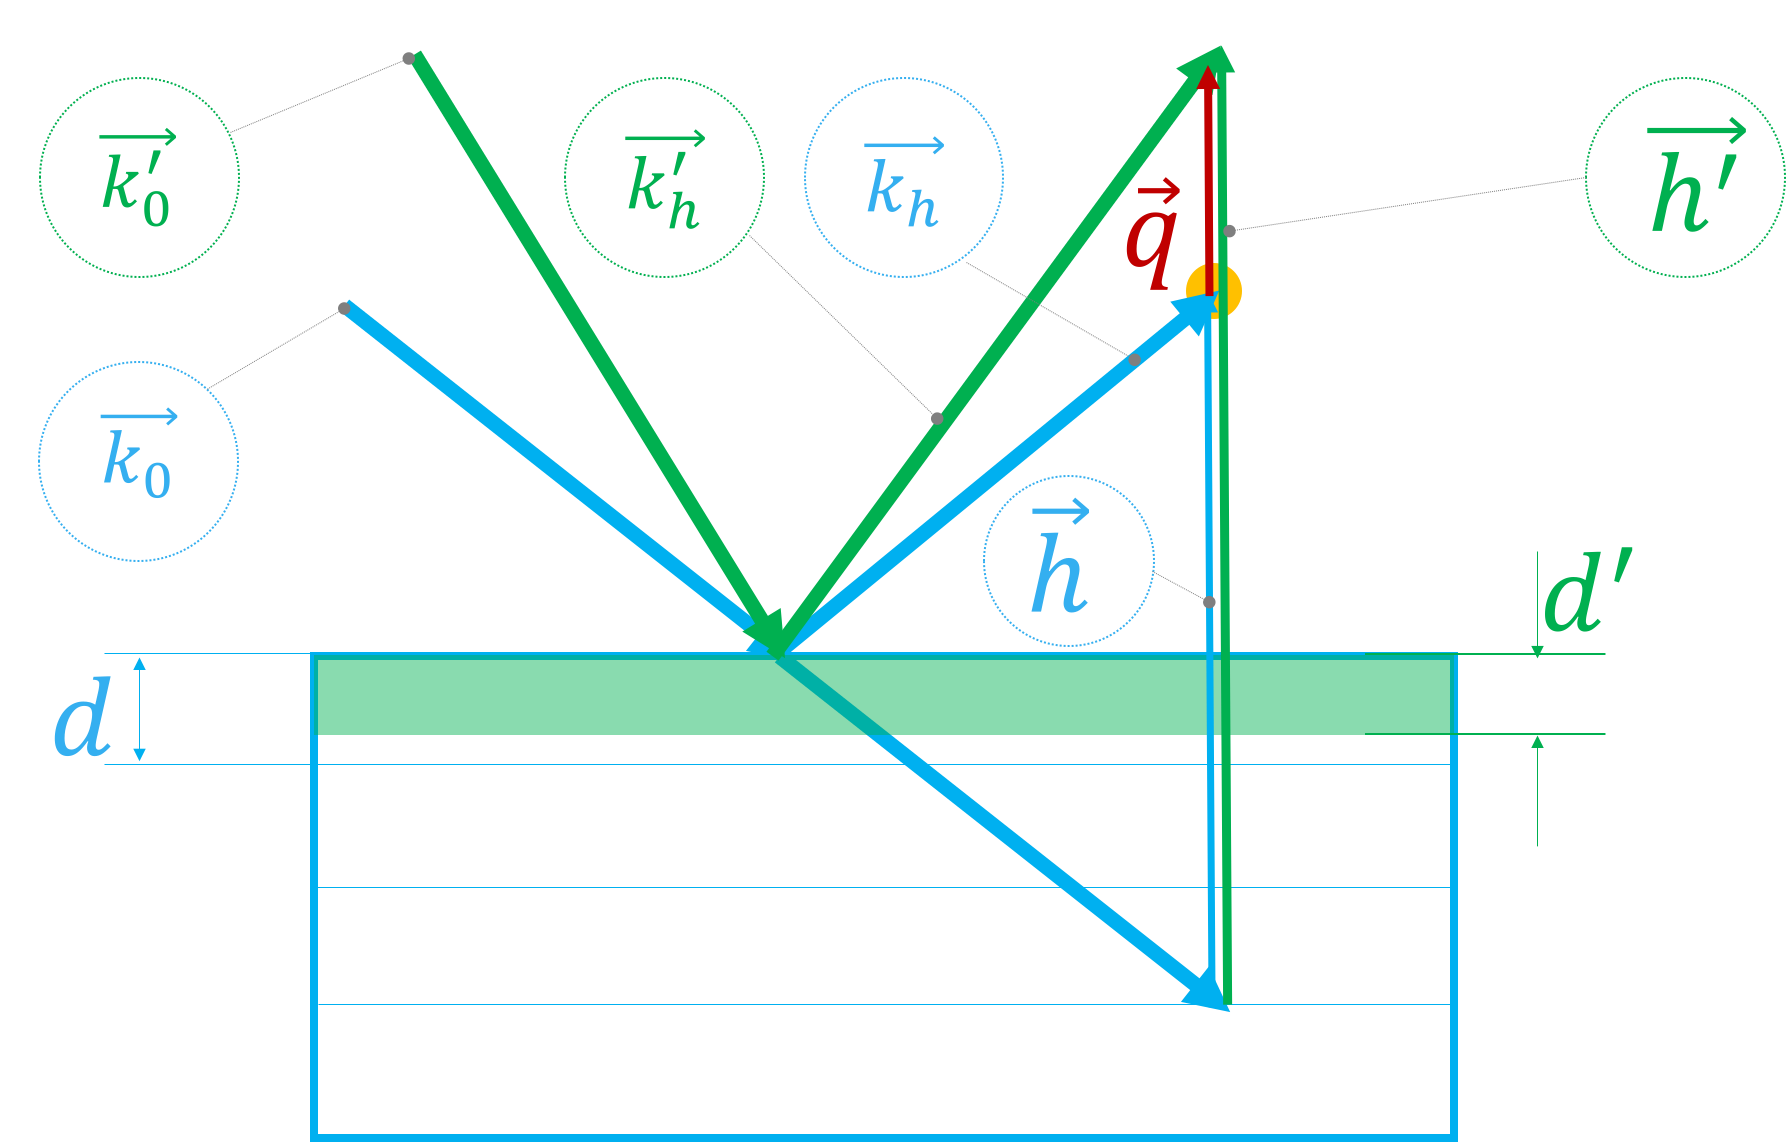
\includegraphics[width=0.3\textwidth]{images/q_vector/_1.png}}
  \hfill
  \subfloat[]{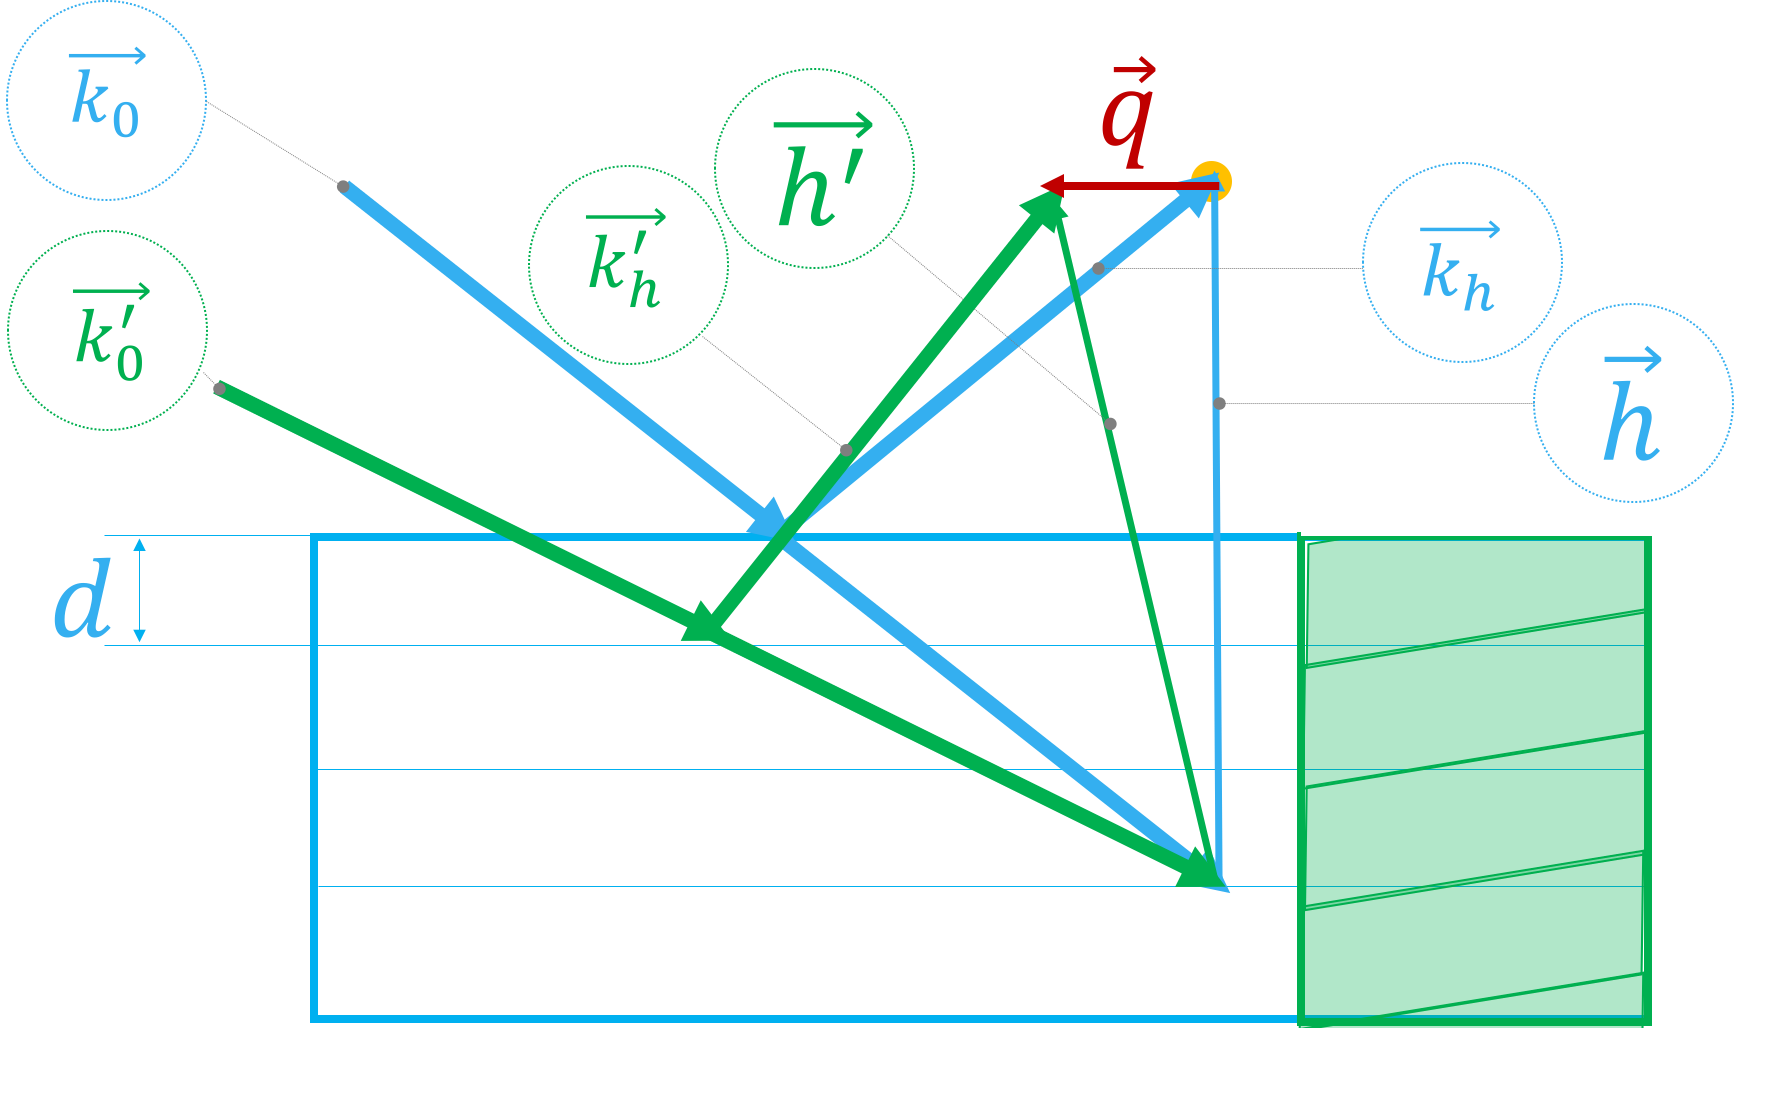
\includegraphics[width=0.3\textwidth]{images/q_vector/1.png}}
  \caption{Отклонение вектора обратной решетки от положения, соответствующего идеальному кристаллу (a),
  при деформации кристаллической решетки (b) и угловой разориентации отражающих плоскостей (с) }
  \label{ris:q_vector_reciprocal_space}
\end{figure}

Для симметричного отражения параметры $q_x$ и $q_z$ связаны с отклонением образца $\theta$ и
анализатора $\varepsilon$ от точного брэгговского положения следующими
уравнениями \cite{Tanner_1998}:

\begin{equation}
  q_x = \frac{\varepsilon}{|\vec{k}_0|} \cos \theta_B,
  \label{eq:qx_eqn}
\end{equation}

\begin{equation}
  q_z = \frac{2\theta - \varepsilon}{|\vec{k}_0|} \sin \theta_B.
  \label{eq:qz_eqn}
\end{equation}

Таким образом, сканирование образцом ($\omega$ - сканирование) влияет только на $q_x$, а
сканирование анализатором ($2\theta$ - сканирование) влияет на обе компоненты,
 изменение только одного $q_z$ достигается за счет $\theta-2\theta$ сканирования.

\begin{figure}[H]
  \centering
  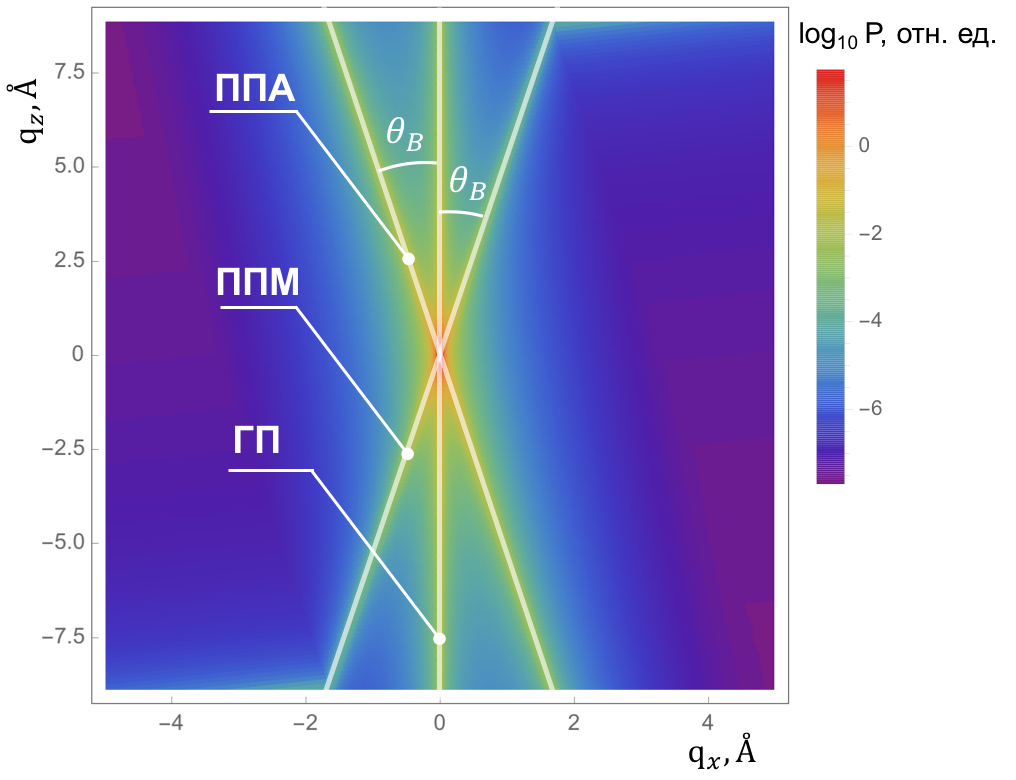
\includegraphics[width=0.6\textwidth]{images/triple_map_reciprocal_space.png}
  \caption{Карта трехкристальной рентгеновской дифракции в обратном пространстве}
  \label{ris:triple_map_reciprocal_space}
\end{figure}

Углы между ППА, ГП и ППМ определяются исходя из соотношений (\ref{eq:qx_eqn}, \ref{eq:qz_eqn}) и равны углу Брэгга образца:
% только ли образца

\begin{equation}
  \frac{q_y}{q_z} = \frac{2\theta - \varepsilon}{\varepsilon} \cdot \tg (\theta_B) = \pm \tg (\theta_B).
  \label{eq:qz_eqn}
\end{equation}
